\section{FFManip Class Reference}
\label{classFFManip}\index{FFManip@{FFManip}}
This class paves the way for mutating the struture of neural networks. 


{\tt \#include $<$FFManip.h$>$}

Inheritance diagram for FFManip::\begin{figure}[H]
\begin{center}
\leavevmode
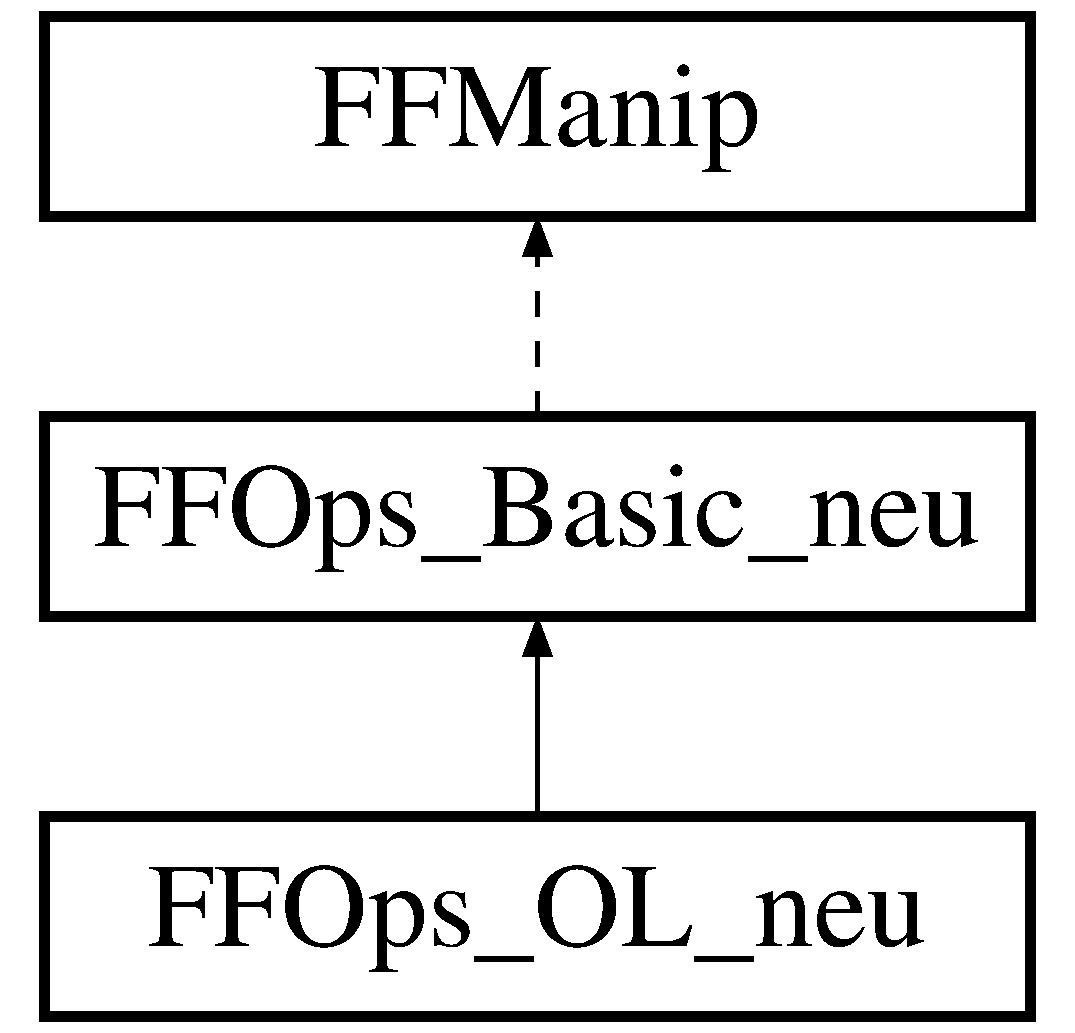
\includegraphics[height=3cm]{classFFManip}
\end{center}
\end{figure}
\subsection*{Protected Methods}
\begin{CompactItemize}
\item 
Array$<$ int $>$ {\bf init\-FFBulk} (const unsigned n\-In, const unsigned n\-Hid, const unsigned n\-Out, const double prob)
\begin{CompactList}\small\item\em initialize the connections randomly of a block of non-layered feedforward neural network\item\end{CompactList}\item 
Array$<$ int $>$ {\bf init\-FFOL} (const unsigned n\-In, const unsigned n\-Hid, const unsigned n\-Out, const double prob1, const double prob2, const double prob3)
\begin{CompactList}\small\item\em initialize the connections randomly of a block of layered feedforward neural network\item\end{CompactList}\item 
void {\bf repair\-Bulk} (Array$<$ int $>$ \&c, const unsigned n\-In, const unsigned n\-Hid, const unsigned n\-Out)
\begin{CompactList}\small\item\em Check if a given neuron structure is valid, otherwise repair it.\item\end{CompactList}\item 
void {\bf repair\-OL} (Array$<$ int $>$ \&c, const unsigned n\-In, const unsigned n\-Hid, const unsigned n\-Out)
\begin{CompactList}\small\item\em Check if a given connection matrix for a layered NN structure is valid.\item\end{CompactList}\item 
void {\bf connect\-New} (Array$<$ int $>$ \&c, Array$<$ double $>$ \&w, unsigned pos, double low, double high)
\begin{CompactList}\small\item\em Add a connection from a given neuron to a randomly selected neuron.\item\end{CompactList}\item 
void {\bf pull\-Through} (Array$<$ int $>$ \&c\-Old, Array$<$ int $>$ \&c, Array$<$ double $>$ \&w, unsigned, double low, double high)
\begin{CompactList}\small\item\em Update connections according to a given matrix to a current one and generate a random weight for that connection.\item\end{CompactList}\item 
\index{max@{max}!FFManip@{FFManip}}\index{FFManip@{FFManip}!max@{max}}
unsigned {\bf max} (unsigned a, unsigned b)\label{classFFManip_b6}

\begin{CompactList}\small\item\em Return {\tt max(a,b)}.\item\end{CompactList}\item 
\index{min@{min}!FFManip@{FFManip}}\index{FFManip@{FFManip}!min@{min}}
unsigned {\bf min} (unsigned a, unsigned b)\label{classFFManip_b7}

\begin{CompactList}\small\item\em Return {\tt min(a,b)}.\item\end{CompactList}\item 
unsigned {\bf n\-Input} (Array$<$ int $>$ \&c, const unsigned N)
\begin{CompactList}\small\item\em Count the number of inputs to a given neuron.\item\end{CompactList}\item 
unsigned {\bf n\-Output} (Array$<$ int $>$ \&c, const unsigned N)
\begin{CompactList}\small\item\em Count the number of outputs to a given neuron.\item\end{CompactList}\item 
Array$<$ unsigned $>$ {\bf dispensable\-FFConnection} (Array$<$ int $>$ \&c, const unsigned n\-In, const unsigned n\-Hid)
\begin{CompactList}\small\item\em Check which connections can be deleted.\item\end{CompactList}\item 
Array$<$ unsigned $>$ {\bf feasible\-FFConnection} (Array$<$ int $>$ \&c, const unsigned n\-In, const unsigned n\-Hid)
\begin{CompactList}\small\item\em Check where a connection can be added.\item\end{CompactList}\end{CompactItemize}


\subsection{Detailed Description}
This class paves the way for mutating the struture of neural networks.

Operations include counting inputs and outputs of a given neuron, checking which neurons or connections could be deleted, and where neurons and connections could be added. 



\subsection{Member Function Documentation}
\index{FFManip@{FFManip}!connectNew@{connectNew}}
\index{connectNew@{connectNew}!FFManip@{FFManip}}
\subsubsection{\setlength{\rightskip}{0pt plus 5cm}void FFManip::connect\-New (Array$<$ int $>$ \& {\em c}, Array$<$ double $>$ \& {\em w}, unsigned {\em pos}, double {\em low}, double {\em high})\hspace{0.3cm}{\tt  [protected]}}\label{classFFManip_b4}


Add a connection from a given neuron to a randomly selected neuron.

The weight for the newly added connection is generated randomly within a given interval \begin{Desc}
\item[Parameters: ]\par
\begin{description}
\item[{\em 
c:}]connection matrix \item[{\em 
w:}]weight matrix \item[{\em 
pos:}]the neuron from which a new connection should be added \item[{\em 
low:}]lower bound of the interval for generating a random weight \item[{\em 
high:}]upper bound of the interval for generating a random weight \end{description}
\end{Desc}
\index{FFManip@{FFManip}!dispensableFFConnection@{dispensableFFConnection}}
\index{dispensableFFConnection@{dispensableFFConnection}!FFManip@{FFManip}}
\subsubsection{\setlength{\rightskip}{0pt plus 5cm}Array$<$unsigned$>$ FFManip::dispensable\-FFConnection (Array$<$ int $>$ \& {\em c}, const unsigned {\em n\-In}, const unsigned {\em n\-Hid})\hspace{0.3cm}{\tt  [protected]}}\label{classFFManip_b10}


Check which connections can be deleted.

A connection can be removed if after deletion, all neurons have at least one input and one output \begin{Desc}
\item[Parameters: ]\par
\begin{description}
\item[{\em 
c:}]connection matrix \item[{\em 
n\-In:}]number of input nodes \item[{\em 
n\-Hid:}]number of hidden nodes \end{description}
\end{Desc}
\index{FFManip@{FFManip}!feasibleFFConnection@{feasibleFFConnection}}
\index{feasibleFFConnection@{feasibleFFConnection}!FFManip@{FFManip}}
\subsubsection{\setlength{\rightskip}{0pt plus 5cm}Array$<$unsigned$>$ FFManip::feasible\-FFConnection (Array$<$ int $>$ \& {\em c}, const unsigned {\em n\-In}, const unsigned {\em n\-Hid})\hspace{0.3cm}{\tt  [protected]}}\label{classFFManip_b11}


Check where a connection can be added.

\begin{Desc}
\item[Parameters: ]\par
\begin{description}
\item[{\em 
c:}]connection matrix \item[{\em 
n\-In:}]number of input nodes \item[{\em 
n\-Hid:}]number of hidden nodes \end{description}
\end{Desc}
\index{FFManip@{FFManip}!initFFBulk@{initFFBulk}}
\index{initFFBulk@{initFFBulk}!FFManip@{FFManip}}
\subsubsection{\setlength{\rightskip}{0pt plus 5cm}Array$<$int$>$ FFManip::init\-FFBulk (const unsigned {\em n\-In}, const unsigned {\em n\-Hid}, const unsigned {\em n\-Out}, const double {\em prob})\hspace{0.3cm}{\tt  [protected]}}\label{classFFManip_b0}


initialize the connections randomly of a block of non-layered feedforward neural network

\begin{Desc}
\item[Parameters: ]\par
\begin{description}
\item[{\em 
n\-In:}]number of input nodes \item[{\em 
n\-Hid:}]number of hidden nodes \item[{\em 
n\-Out:}]number of output nodes \item[{\em 
prob:}]probability for a connection \end{description}
\end{Desc}
\index{FFManip@{FFManip}!initFFOL@{initFFOL}}
\index{initFFOL@{initFFOL}!FFManip@{FFManip}}
\subsubsection{\setlength{\rightskip}{0pt plus 5cm}Array$<$int$>$ FFManip::init\-FFOL (const unsigned {\em n\-In}, const unsigned {\em n\-Hid}, const unsigned {\em n\-Out}, const double {\em prob1}, const double {\em prob2}, const double {\em prob3})\hspace{0.3cm}{\tt  [protected]}}\label{classFFManip_b1}


initialize the connections randomly of a block of layered feedforward neural network

\begin{Desc}
\item[Parameters: ]\par
\begin{description}
\item[{\em 
n\-In:}]number of input nodes \item[{\em 
n\-Hid:}]number of hidden nodes \item[{\em 
n\-Out:}]number of output nodes \item[{\em 
prob1:}]probability for a connection between input and hidden nodes \item[{\em 
prob2:}]probability for a connection between hidden and output nodes \item[{\em 
prob3:}]probability for a connection between bias nodes and other nodes \end{description}
\end{Desc}
\index{FFManip@{FFManip}!nInput@{nInput}}
\index{nInput@{nInput}!FFManip@{FFManip}}
\subsubsection{\setlength{\rightskip}{0pt plus 5cm}unsigned FFManip::n\-Input (Array$<$ int $>$ \& {\em c}, const unsigned {\em N})\hspace{0.3cm}{\tt  [protected]}}\label{classFFManip_b8}


Count the number of inputs to a given neuron.

\begin{Desc}
\item[Parameters: ]\par
\begin{description}
\item[{\em 
c:}]connection matrix \item[{\em 
N:}]the neuron whose inputs are to be counted \end{description}
\end{Desc}
\index{FFManip@{FFManip}!nOutput@{nOutput}}
\index{nOutput@{nOutput}!FFManip@{FFManip}}
\subsubsection{\setlength{\rightskip}{0pt plus 5cm}unsigned FFManip::n\-Output (Array$<$ int $>$ \& {\em c}, const unsigned {\em N})\hspace{0.3cm}{\tt  [protected]}}\label{classFFManip_b9}


Count the number of outputs to a given neuron.

\begin{Desc}
\item[Parameters: ]\par
\begin{description}
\item[{\em 
c:}]connection matrix \item[{\em 
N:}]the neuron whose outputs are to be counted \end{description}
\end{Desc}
\index{FFManip@{FFManip}!pullThrough@{pullThrough}}
\index{pullThrough@{pullThrough}!FFManip@{FFManip}}
\subsubsection{\setlength{\rightskip}{0pt plus 5cm}void FFManip::pull\-Through (Array$<$ int $>$ \& {\em c\-Old}, Array$<$ int $>$ \& {\em c}, Array$<$ double $>$ \& {\em w}, unsigned, double {\em low}, double {\em high})\hspace{0.3cm}{\tt  [protected]}}\label{classFFManip_b5}


Update connections according to a given matrix to a current one and generate a random weight for that connection.

\begin{Desc}
\item[Parameters: ]\par
\begin{description}
\item[{\em 
c\-Old:}]the old connection matrix \item[{\em 
c:}]the new connection matrix  \item[{\em 
w:}]the weight matrix \item[{\em 
low:}]lower bound of the interval for generating a random weight \item[{\em 
high:}]upper bound of the interval for generating a random weight \end{description}
\end{Desc}
\index{FFManip@{FFManip}!repairBulk@{repairBulk}}
\index{repairBulk@{repairBulk}!FFManip@{FFManip}}
\subsubsection{\setlength{\rightskip}{0pt plus 5cm}void FFManip::repair\-Bulk (Array$<$ int $>$ \& {\em c}, const unsigned {\em n\-In}, const unsigned {\em n\-Hid}, const unsigned {\em n\-Out})\hspace{0.3cm}{\tt  [protected]}}\label{classFFManip_b2}


Check if a given neuron structure is valid, otherwise repair it.

\begin{Desc}
\item[Parameters: ]\par
\begin{description}
\item[{\em 
c:}]a connection matrix to be checked \item[{\em 
n\-In:}]number of input nodes \item[{\em 
n\-Hid:}]number of hidden nodes \item[{\em 
n\-Out:}]number of output nodes \end{description}
\end{Desc}
\index{FFManip@{FFManip}!repairOL@{repairOL}}
\index{repairOL@{repairOL}!FFManip@{FFManip}}
\subsubsection{\setlength{\rightskip}{0pt plus 5cm}void FFManip::repair\-OL (Array$<$ int $>$ \& {\em c}, const unsigned {\em n\-In}, const unsigned {\em n\-Hid}, const unsigned {\em n\-Out})\hspace{0.3cm}{\tt  [protected]}}\label{classFFManip_b3}


Check if a given connection matrix for a layered NN structure is valid.

\begin{Desc}
\item[Parameters: ]\par
\begin{description}
\item[{\em 
c:}]a connection matrix to be checked \item[{\em 
n\-In:}]number of input nodes \item[{\em 
n\-Hid:}]number of hidden nodes \item[{\em 
n\-Out:}]number of output nodes \end{description}
\end{Desc}


The documentation for this class was generated from the following file:\begin{CompactItemize}
\item 
FFManip.h\end{CompactItemize}
